%!TEX root = main.tex

\section{Introduction}

\noindent A key challenge facing Internet services today is how to share resources across users to maximize the user-perceived {\em QoE} (Quality of Experience) by minimizing their end-to-end delay.
Maintaining a desirable level of user-perceived QoE is critical because reducing a few hundred milliseconds from the page load time means millions of dollars.
%The fundamental challenge facing large-scale web service providers and (\eg Microsoft, Facebook, Akamai, Google, Amazon) is how the backend systems should share its resources in order to optimize user-perceived {\em QoE} (Quality of Experience). 
%Maintaining desirable level of user-perceived QoE critical for their revenue models.
A delay penalty of 400ms in Google search responses reduces search volume by 0.74\%; and 500ms of latency for Bing decreases revenue by 1.2\%~\cite{google-revenue,bing-revenue}; For Amazon, an additional latency of 100ms means a 1\% drop in sales~\cite{amazon-revenue}.
Yet, despite substantial efforts (\eg~\cite{shandian,gaze,rosen2017push,jalaparti2013speeding}), maintaining desirable QoE remains a challenge, with average page loading time of Facebook requests being over 3000ms~\cite{mystery}.
% with 50\% users of some popular website spending over 30\% of page loading time on the web backend~\cite{mystery}.

We argue that the key missing piece of today's Internet architecture is that individual Internet systems, \eg web backends, CDNs, and ISPs, are oblivious to their impact on individual users' real-time QoE, especially when the impacts vary across users.
As a consequence, it is difficult for these systems to directly optimize QoE. 
Instead, our overarching thesis is that these systems should be driven directly by the real-time information about their impact on the QoE across users, which could substantially improve QoE as well as resource efficiency, without adding new resources.
While there have been similar efforts in the past (\eg~\cite{alto,frank2013pushing,xie2008p4p,jiang2009cooperative}) toward similar end-to-end and cross-layer optimization, our project is inspired by several favorable recent trends, including ``use-case pulls'', such as the prevalence of QoE-driven revenue models (\eg~\cite{akamai-report,dobrian2011understanding}), as well as ``technological pushes'', such as the wide use of tracing from the clients and the backend systems (\eg~\cite{mystery,zhao2014lprof}). 

This proposal explores the benefits and challenges of our thesis in the context of how web backend systems should optimize web QoE by leveraging user heterogeneity. 

\mypara{Limitation of today's web backend}
%The web backend systems today have no direct visibility of the QoE of each web request when it arrives, 
Because the end-to-end delay (page loading time) of a web request is affected by the delay of many non-backend systems (ISPs, client-side software, etc) that are beyond the scope of the web service providers, the web backend systems have no direct visibility of how much impact it has on the QoE of individual requests.
As a result, the web backend systems seek to minimize the overall {\em backend delay} (\eg the mean, tail values, or the probability of missing some SLA deadline), under the assumption that backend delay of $n$~ms has the {\em same} impact on any request.\footnote{Modulo the content-specific (\eg web page type) or user-specific (\eg free vs. premium subscription) factors.}
%Page load time, which we refer to as {\em end-to-end delay}, generally consists of three parts: client-side delay, wide-area network (WANs) delay, and backend delay.
%- Web services, like applications running in the cloud, have been basing their optimizations on the goal of improving server-side latency (sometimes the fraction of users meeting some fixed deadline)
%Because of the federated nature of Internet architecture, web service providers do not have full control over all types of delays.
%---to them, WANs and clients devices are largely blackboxes operated, not by the web services, but by ISPs, cellular carriers, and device vendors.
%(while web browsers and apps are developed by the web service providers, the client-side performance is largely decided by how OS share resources among multiple applications).
%With web service providers only controlling the web backend, the performance metric they focus on optimizing is the 
%%Thus, instead of optimizing for QoE directly, today's web services focus on reducing the 
%%different requests have the same {\em QoE sensitivity to backend delay}
%{\em backend delay}, under the assumption that a backend delay of $n$~ms has the {\em same} impact on any request.\footnote{Modulo the content-specific (\eg web page type) or user-specific (\eg free vs. premium subscription) factors.}
% That is, a backend delay of $n$~ms has the same effect on the QoE of any request.
%For instance, they minimize the mean/tail backend delay or the fraction of requests whose backend delay exceeds some deadline (\eg 300ms)~\cite{??,??}.
%- This project takes a step back and asks a different question: does the latency have the same impact on user QoE? 
% In doing so, 
%all requests are optimized with the same objective function of backend response time; 
% an implicit assumption is that different requests have the same {\em QoE sensitivity to backend delay} (modulo content-/user-specific factors, such as web page type or subscription type, etc);
% that is, a backend delay of $n$~ms has the same effect on the QoE of different requests.

We take a step back, and ask {\em ``does the backend delay really have the same impact on the QoE of any web request?''}
%- The answer is no, which has profound impact on how web services should be built. [Give a simple example here.] In essence, this means giving each ``priority'', in terms of resources and scheduling, is cost-inefficient and suboptimal. [Give a simple example. resources wasted for users who are screwed already]
Our answer is {\em no}, and such heterogeneous sensitivity of QoE to backend delay is pervasive among requests of the same application. 
This is due to the fact that how much impact the backend delay has on a request depends on the non-backend delay experienced by a request (\eg ISP routing, client-side resource allocation by the device OS), which can have great variability among requests and over time~\cite{timecard,dqbarge}.
%Two observations contribute to this conclusion: the non-linear relationship between page load time and QoE~\cite{??} and the fact that the WAN/client delay varies among requests~\cite{timecard,dqbarge}, {\em the QoE sensitivity to backend delay varies among requests.}
For instance, the QoE of a web request that has spent 50ms on wide-area networks tends to be more sensitive to 10ms backend delay than a request that has already spent 500ms on the network.
By falsely assuming requests are equally sensitive to the backend delay, traditional web backend system (Figure~\ref{fig:intro-overview}(a)) might waste resources on requests that are insensitive to the backend delay, and/or have suboptimal QoE (\eg using inadequate resources on requests whose QoE is critically dependent on the backend delay. 

\mypara{Our approach} 
We introduce ``QoE sensitivity'' as a new dimension for web QoE optimization, and propose to develop {\bf QoE-driven web backend} systems (Figure~\ref{fig:intro-overview}(b)). 
We argue that embracing the heterogeneity in QoE's sensitivity to backend delay has profound implications for backend systems: 
it should allocate resources in a way that favors the requests whose QoE is more sensitive to backend delay to improve the overall QoE while having only a minimal drop in the QoE of other requests.
For instance, in a trace-driven simulation (\S\ref{sec:quantifying}), we found that a simple QoE-driven resource allocation policy can raise user experience (measured in user engagement) 50\% closer to optimal (\ie zero backend delay) than a QoE-agnostic reference web backend.
%should allocate their limited resources. 
%By taking into account the QoE's sensitivity to the backend delay, 
%\jc{bring up some concrete improvement numbers}
%\jc{need to highlight that this is not because application differents}

\begin{figure}[t]
	\centering
	\vspace{-0.5cm}
%	\hspace{0.6cm}
	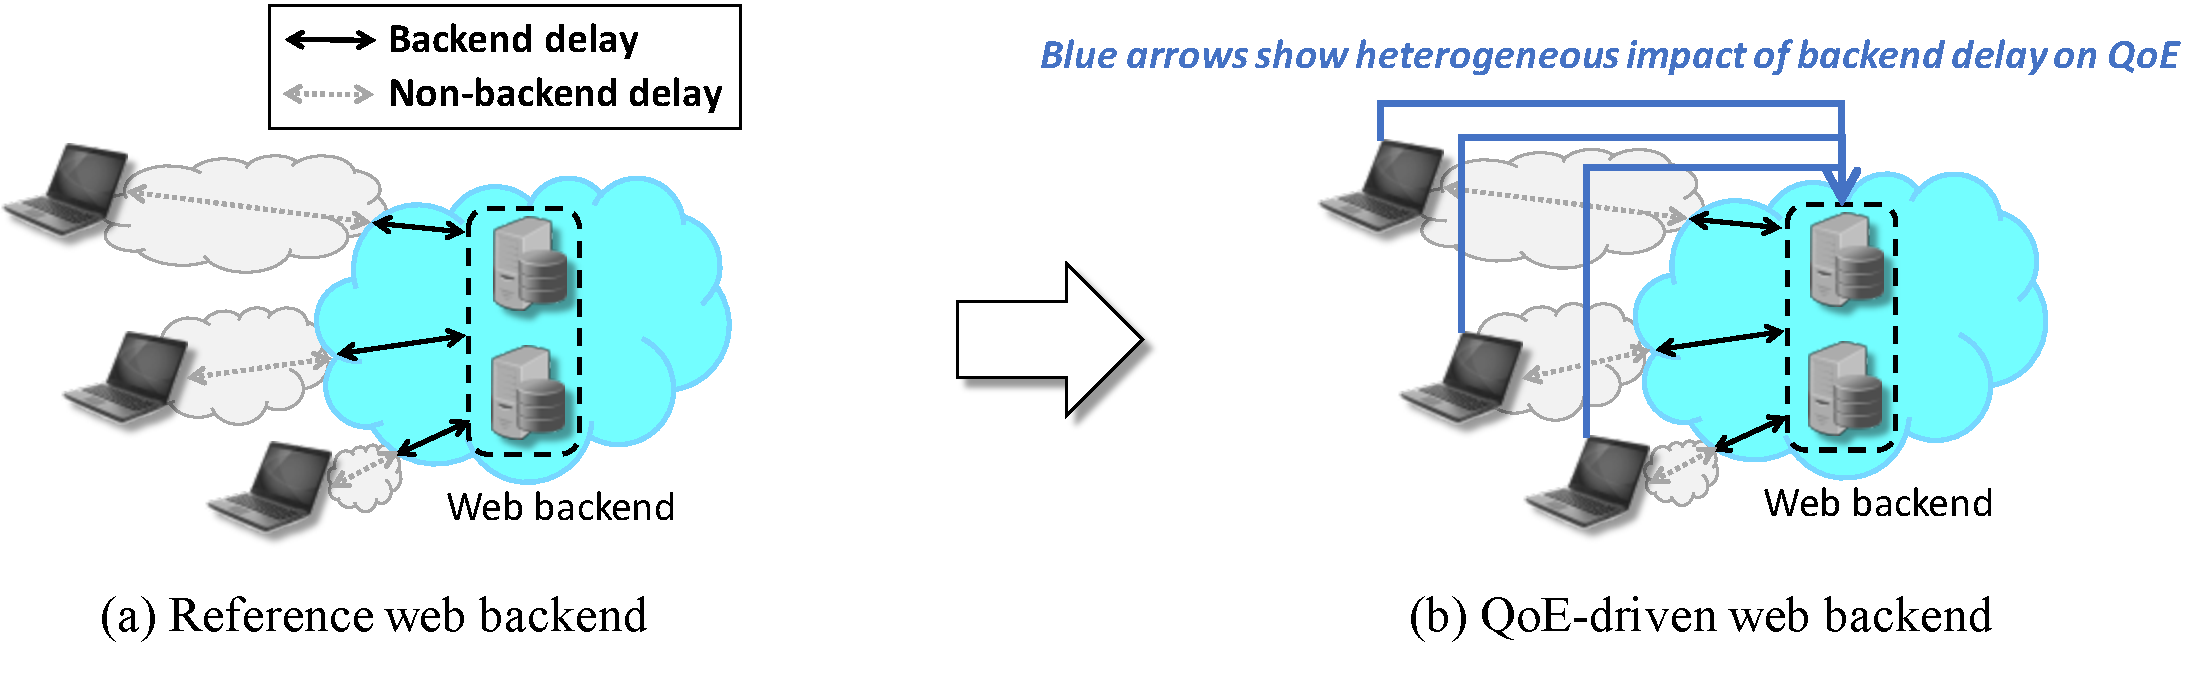
\includegraphics[width=0.8\textwidth]{figs/intro-overview-new.pdf}
	\vspace{-0.4cm}
	\caption{We propose to re-architect (a) today's web backend which seeks to minimize the backend delays into (b) a QoE-driven web backend which seeks to minimize the {\em impact of backend delay on QoE}.}
	\label{fig:intro-overview}
\end{figure}

%\jc{give a figure to contrast optimization of backend in-isolation vs. QoE-aware.}

%- Research goal: This project proposes that the web service backend should be aware of the QoE sensitivity. This effectively changes how one formulates the web service optimization problem.


%The key difference is that 
%Unlike a traditional backend which seeks to minimize the backend delays, a QoE-driven backend seeks to minimize the impact of backend delays on user-perceived QoE.

Despite its promise, we face two key challenges.
First, when a request is received, the backend needs to estimate in real time the sensitivity of the request's QoE to the backend delay with sufficient accuracy, and propagate the information across individual components of the backend. This information is not readily available in today's backend.
Second, the resource allocation and scheduling logic of web backend subsystems need to be updated to leverage the heterogeneity across users. The challenge arises from the fact that requests need to be set with different priorities in real time depending on their non-backend delay.
There are other problem inherent to the QoE-driven approach, including control stability (\ie the backend system becomes sensitive to any changes in non-backend delay), and exacerbating QoE unfairness (\ie the backend system favors sensitive users who may already have better QoE than some others).
%Through developing novel algorithms and architectural components, we show that a {\bf QoE-driven web backend} (Figure~\ref{fig:intro-overview}(b)), which is aware of and embraces the differences of QoE sensitivity across requests, can substantially {\em improve the resource/QoE tradeoffs} of web backend; \ie better QoE without using more resources, or saving resources without degrading QoE. 
% Note that being QoE sensitivity does not require expensive infrastructure changes (\eg adding hardware or changing software stack).

\mypara{Research plan}
We will explores the problem space by focusing on addressing the first two challenges, and will also discuss other questions (\eg control instability and unfairness).
We divide the proposed research into three main tasks. 
%We use the following roadmap to thoroughly examine the benefits and challenges of QoE-sensitivity-aware web service backend.

\begin{packedenumerate}
\item{\bf Quantifying potential benefits (Task \#1).}
We will use a mix of user studies and analysis of industry datasets to quantify the potential improvement (in terms of QoE and resource savings) brought by the QoE-driven web backend in real-world workloads and identify the opportunities of QoE-driven optimizations in existing web backend systems.%, and use measurement dataset from large-scale web services to understand its potential in the real-world traffic patterns.

\item{\bf Estimating backend's impact on per-request QoE in real time (Task \#2).}
We will develop new tracing infrastructure and QoE prediction models to estimate the impact of backend delay on requests' QoE in real time. We will investigate the possibilities of incremental deployment by reusing the existing tracing and telemetry infrastructure in today's web backend systems.

\item{\bf Designing QoE-driven control algorithms (Task \#3).}
We will develop novel control policies for web backend, including scheduling, and replica selection, to leverage the user heterogeneity. Our design objectives are: (1) it should achieve near-optimal QoE with minimal decision-making overhead, and (2) the implementation should be amenable to existing systems.

\end{packedenumerate}


\mypara{PI qualification}
The PI's expertise includes computer networking, Internet QoE, and data analytics systems.
He has published 11 peer-reviewed research papers (6 first-authored) in top-tier networking and systems conferences (\ie SIGCOMM, NSDI, CoNEXT).
More importantly, the PI has a deep understanding of Internet QoE. His doctoral dissertation, titled ``Enabling Data-Driven Optimization of Quality of Experience in Internet Applications,'' is among the first systematic applications of data-driven approach to improving Internet QoE, and some of the proposed QoE prediction techniques (\eg~\cite{cfa,c3}) have led to real-world deployment and impact. The dissertation won the CMU SCS Doctoral Dissertation Award and was nominated for ACM Dissertation Award.
%During his PhD and postdoctoral years, 
He has extensive collaborations with Microsoft, Conviva, and Google, which will help the proposed research gain insights from the industry and provide viable paths to deployment.
%These strong connection

%This project will provide the material needed for further research on the QoE-driven systems and is part of the necessary and critical steps for the PI to achieve research independence.

\mypara{Prior NSF support} The PI has had no prior NSF support.

This project will provide preliminary results on potentials and feasibility of a QoE-driven web backend, which will allow us to further apply similar approach to other Internet systems. This is part of the necessary steps for the PI to achieve research independence.

%\newpage









